\documentclass[12pt, aspectratio=169]{beamer}

\input{../header}
% \usepackage{booktabs}
% \usepackage{tikz}
% \usetikzlibrary{patterns}
\DeclareMathOperator{\E}{E}
\DeclareMathOperator{\Var}{Var}
\DeclareMathOperator{\V}{V}
\DeclareMathOperator{\C}{C}


\title{Random Variable and Probabiilty Distribution}
\author{Md. Aminul Islam Shazid}
\date{}


\begin{document}
    {
		\setbeamertemplate{footline}{}    % NO FOOTLINE FOR THESE TWO FRAMES
		\addtocounter{framenumber}{-2}    % not counting the title page and the outline in frame numbers

		\begin{frame}
			\titlepage
		\end{frame}

		\begin{frame}{Outline}
            \vfill
			\tableofcontents[subsectionstyle=hide]
            \vfill
		\end{frame}
	}


	\section{Probability Distribution}

	\begin{frame}{Probability Distribution}
		\begin{itemize}
			\item A variable which takes numerical values resulting from random experiments, is called a random variable (RV).
			\item Recall that probability distribution means the distribution of the probabilities among the different values of a random variable
		\end{itemize}
			There are some distributions that often arise frequently in real life. This slide shall discuss a few such distributions
	\end{frame}


	\begin{frame}{Types of Probability Distribution}
		Recall that depending on the type of variable, distributions are of two types:
		\begin{itemize}
			\item \textbf{Discrete probability distribution}: probability distribution of a discrete random variable
			\item \textbf{Continuous probability distribution}: probability distribution of a continuous random variable
		\end{itemize}
	\end{frame}


	\begin{frame}{Probability Mass/Density Functions}
		\begin{itemize}
			\item The probability distribution of a discrete random variable is given by its probability mass function (PMF)
			\begin{itemize}
				\item Denoted by \(p(x)\), it gives the probability \(P(X = x)\)
			\end{itemize}
			\item The probability distribution of a continuous random variable is given by its probability density function (PDF)
				\begin{itemize}
					\item Denoted by \(f(x)\)
					\item \(\displaystyle \int_a^b f(x) \, dx = P(a < X < b)\)
				\end{itemize}
		\end{itemize}
		Only for the continuous case: \(P(X = k) = 0\), where \(k\) is some constant.
	\end{frame}


	\begin{frame}{Cumulative Distribution Function (CDF)}
				\begin{itemize}
			\item For discrete random variable, \(
				F(x) = P(X \leqslant x) = \displaystyle \sum_{k=-\infty}^{x} p(k)
			\)
			\item For continuous case, \(
				F(x) = P(X \leqslant x) = P(X<x) = \displaystyle \int_{-\infty}^{x} f(x) \, dx
			\)
			\item It is a non-decreasing function, the largest value \(F(x)\) can take is \(1\)
		\end{itemize}

		\vspace{0.5em}

		Here, summing/integrating from $-\infty$ means that the lower limit of the sum/integral is the smallest value in the domain of the random variable $X$.
	\end{frame}


	\section{Some Common Discrete Probability Distributions}

	\subsection{Bernoulli and Binomial Distributions}

	\begin{frame}{Bernoulli Process}
		When a random process or experiment, called a trial, can result in only one of two mutually exclusive outcomes, such as dead or alive, sick or well, full-term or premature, the trial is called a Bernoulli trial.

		\begin{itemize}
			\item Each trial results in one of two possible, mutually exclusive, outcomes. One of the possible outcomes is denoted (arbitrarily) as a success, and the other is denoted a failure
			\item The probability of a success, denoted by $p$, remains constant from trial to trial. The probability of a failure, $1 - p$, is denoted by $q$
			\item The trials are independent; that is, the outcome of any particular trial is not affected by the outcome of any other trial
		\end{itemize}
	\end{frame}


	\begin{frame}{Bernoulli Distribution}
		Let $X$ be the number of successe in a single Bernoulli trial. Then $X$ follows a Bernoulli distribution. It is written as:
		\[X \sim \mathrm{Bernoulli}(p).\]

		The probability mass function (PMF) of $X$ is given as:
		\[
			p(x) = p^x (1-p)^{1-x} \, ; \quad x = 0, 1
		\]

		\begin{itemize}
			\item Expected value, \(\E(X) = 1 \times p + 0 \times (1-p) = p\)
			\item Variance: \begin{align*}
				\V(X) = \E(X^2) - [\E(X)]^2 &= (1^2 \times p + 0^2 \times (1-p)) - p^2 \\
				 &= p - p^2 = p(1-p)
			\end{align*}
		\end{itemize}
	\end{frame}


	\begin{frame}{Binomial Distribution}
		Let $X$ be the number of successes in $n$ Bernoulli trials, where the probability of success is $p$. Then the random variable $X$ follows a binomial distribution. It is written as:
		\[X \sim \mathrm{binom}(n, p).\]

		The probability mass function (PMF) of $X$ is given as:
		\[
			p(x) = ^n\C_x \, p^x (1-p)^{n-x} \, ; \quad x = 0, 1, 2, 3...
		\]

		\begin{itemize}
			\item \(\E(X) = np\)
			\item \(\V(X) = np(1-p)\)
		\end{itemize}
	\end{frame}


	\begin{frame}{Binomial Distribution: Shape}
		\centering
		
\includegraphics[width=\textwidth]{plots/binomial-shape.pdf}
	\end{frame}


	\begin{frame}{Examples of Binomial Variables}
		\begin{itemize}
			\item Number of defective products among a batch of products
			\item Number of patients carrying a ceratain pathogen among a group of patients
			\item Number of heads when a coin is tossed several times
		\end{itemize}
	\end{frame}


	\begin{frame}{Binomial Distribution: Example}
		There are 3 multiple choice questions in a MCQ test. Each MCQ consists of four possible choices and only one of them is correct. If an examinee answers those MCQ randomly (without knowing the correct answers).
		\begin{enumerate}
			\item What is the probability that exactly any two of the answers will be correct?
			\item What is the probability that at least two of the answers will be correct?
			\item What is the probability that at most two of the answers will be correct?
			\item What will be the average or expected number of correct answers?
			\item Also, find the standard deviation of number of correct answers.
		\end{enumerate}
	\end{frame}


	\begin{frame}{Binomial Distribution: Example Solution}
		Each MCQ has $4$ options. So, when answering randomly, probability of correct answer, $p = 1/4 = 0.25$.
		Let the random variable $X$ denote the number of correct answers. Then, \(X \sim \mathrm{binomial}(3, 0.25)\).

		\begin{enumerate}
			\item Probability of two correct answers, \(P(X=2) = ^3\C_2 \, 0.25^2 \, (1-0.25)^{3-2}\)
			\item Probability of \emph{at least} two correct answers \(=P(X=2) + P(X=3)\)
			\item Probability of \emph{at most} two correct answers \(=P(X=0) + P(X=1) + P(X=2)\)
			\item Expected number of correct answers, \(\E(X) = 3 \times 0.25 = 0.75\)
			\item Variance of number of correct answers, \(\V(X) = 3 \times 0.25 \times (1-0.25)\)
		\end{enumerate}

		The calculations for question 2 and 3, are left as exercises.
	\end{frame}


	\subsection{Poisson Distribution}

	\begin{frame}{Poisson Distribution}
		A Poisson random variable is a discrete random variable that counts the number of times a certain event occurs within fixed interval of time, or area, or volume or any other unit.

		\vspace{0.5em}
		
		The Poisson distribution describes the probability of these counts.

		\vspace{0.5em}

		Let \(X ~ \sim \mathrm{Poisson}(\lambda)\), then the PMF of $X$ is given by:
		\[
			P(X=x) = \frac{e^{-\lambda} \lambda^x}{x!} \,; \quad \lambda > 0; \, \quad x=0, 1, 2, 3,...
		\]

		\begin{itemize}
			\item $\lambda$ is the parameter of the distribution
			\item \(\E(X)=\lambda\)
			\item \(\V(X)=\lambda\)
		\end{itemize}
	\end{frame}


	\begin{frame}{Examples of Poisson Random Variables}
		\begin{itemize}
			\item Number of phone calls received by a call center in one minute
			\item Number of typing errors on a page of text
			\item Number of accidents at an intersection in a day
			\item Number of emails arriving in an hour
		\end{itemize}
	\end{frame}


	\begin{frame}{Poisson Distribution: Shape}
		\centering
		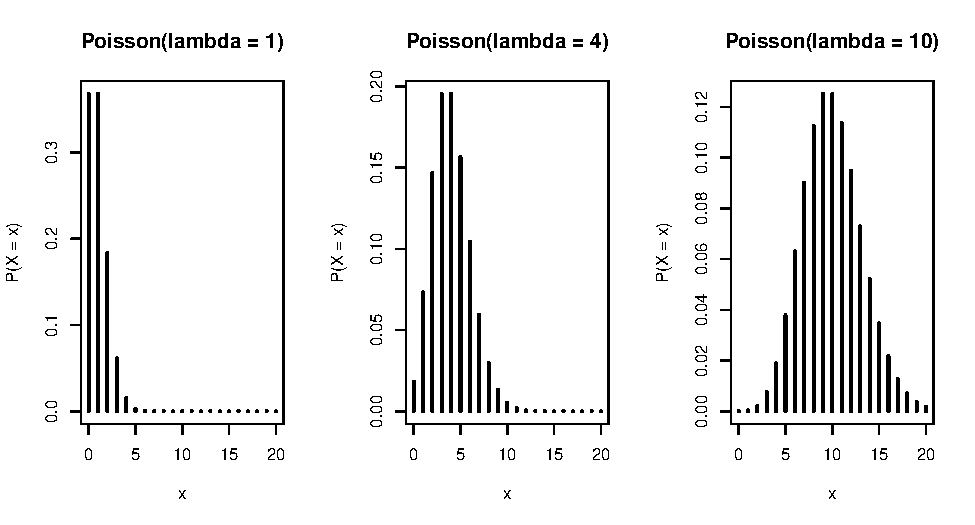
\includegraphics[width=\textwidth]{plots/poisson_shapes.pdf}
	\end{frame}


	\begin{frame}{Assumptions of a Poisson Process}
		\begin{itemize}
			\item Events occur independently of each other
			\item The probability of more than one event in a very small interval is negligible
			\item The average rate of occurrence $\lambda$ is constant over the interval
			\item The probability of an event occurring is proportional to the length of the interval
		\end{itemize}
	\end{frame}


	\begin{frame}{Poisson Distribution: Example}
		The average number of errors on a page of a certain magazine is $0.2$. What is the probability that:
		\begin{enumerate}
			\item a randomly selected page contains $0$ (zero) error?
			\item a randomly selected page contains $2$ or more errors?
			\item two consecutive pages have $3$ errors?
			\item What is the average error per page?
			\item Also, find standard deviation of the number of errors in a page.
		\end{enumerate}
	\end{frame}


	\begin{frame}{Poisson Distribution: Example Solution}
		Here, error rate, \(\lambda = 0.2\).
		\begin{enumerate}
			\item Probability that a randomly selected page contains $0$ errors is 
			\[
				P(X=0) = \frac{e^{-0.2} \, 0.2^0}{0!}
			\]
			\item Probability that a randomly selected page contains $2$ or more errors is
			\begin{align*}
				P(X \geqslant 2) &= 1 - P(X < 2) \\
				&= 1 - [P(X=0) + P(X=1)]
			\end{align*}
		\end{enumerate}
		The above calculations are left as an exercise.
	\end{frame}


	\begin{frame}{Poisson Distribution: Example Solution (cont.)}
		
		\begin{enumerate}
			\setcounter{enumi}{2}
			\item Probability that two consecutive pages have $3$ errors:
			
			\vspace{0.25em}
			
			The error rate for two pages is, \(\lambda_{\mathrm{new}} = 0.2 \times 2 = 0.4\)/

			\vspace{0.25em}

			Therefore, the desired probability is:
			\[
				\frac{e^{-0.4} \, 0.4^3}{3!}.
			\]

			\item Average error per page is \(\E(X) = \lambda = 0.2\).
			\item Standard deviation of number of errors in a page, \(\operatorname{SD}(X) = \sqrt{\V(X)} = \sqrt{0.2}\).
		\end{enumerate}
	\end{frame}


	% \begin{frame}{Geometric Distribution}
		
	% \end{frame}


	\section{Some Common Continuous Probability Distributions}

	\subsection{Uniform Distribution}

	\begin{frame}{Uniform Distribution}
		A random variable with equal probability for all the possible values it can take, is called a uniform random variable.

		\vspace{0.5em}

		Let \(X\) be a uniformly distributed random variable in \([a, b]\), it is written mathematically as \(X \sim \mathrm{uniform}(a, b)\).

		\vspace{0.5em}
		
		The PDF of \(X\) is given by:
		\[
			f(X) = \frac{1}{b-a} \, ; \quad a \leqslant x \leqslant b
		\]

		\begin{itemize}
			\item \(\E(X) = \frac{1}{b-a}\)
			\item \(\V(X) = \frac{(b-a)^2}{12}\)
		\end{itemize}
	\end{frame}


	\begin{frame}{Uniform Distribution: Shape}
		\centering
		
\includegraphics[width=\textwidth]{plots/uniform_shapes.pdf}
	\end{frame}


	\begin{frame}{Uniform Distribution: Example}
		The waiting time (in minutes) for train is uniform($10, 50$). Find the following:
		\begin{enumerate}
			\item The probability that you have to wait at least $20$ minutes
			\item Average waiting time
			\item Standard deviation of waiting time
		\end{enumerate}
	\end{frame}


	\begin{frame}{Uniform Distribution: Example Solution}
		Here, wait time, \(X \sim \mathrm{uniform}(10, 50)\)
		\begin{enumerate}
			\item Probability of waiting at least 20 minutes:
			\begin{align*}
				P(X>20) = P(20 \leqslant X \leqslant 50) &= \int_{20}^{50} \frac{1}{50-10}\\
				&= \Big[\frac{x}{40}\Big]_{20}^{50} = 30/40
			\end{align*}

			\item Average waiting time, \(\E(X) = \frac{10 + 50}{2} = 30\)
		\end{enumerate}

		\vspace{0.5em}

		Question 3 is left as an exercise.
	\end{frame}


	\subsection{Exponential Distribution}

	\begin{frame}{Exponential Distribution}
		Let \(X\) be a continuous random variable measuring the waiting time until an event occurs. The event is assumed to occur randomly but at a constant average rate. And let \(\lambda\) be the average number of events in one unit of time.

		\vspace{0.5em}

		Then \(X\) is said to follow the exponential distribution with rate parameter \(\lambda\), written as \(X \sim \mathrm{exponential}(\lambda)\).

		\vspace{0.5em}

		The PDF of \(X\) is given by 
		\[
			f(x) = \lambda e^{-\lambda x} \,; \quad x> 0, \quad \lambda > 0.
		\]

		\begin{itemize}
			\item \(E(X) = 1/\lambda\), it denotes the average waiting time between events
			\item \(\V(X) = 1/\lambda^2\)
		\end{itemize}
	\end{frame}


	\begin{frame}{Examples of Exponentially Distributed Random Variables}
		\begin{itemize}
			\item Waiting time until the next customer arrives at a service counter
			\item Time between two consecutive phone calls arriving at a call center
			\item Lifetime of an electronic component assuming a constant failure rate
			\item Time until a radioactive atom decays
			\item Waiting time until the next bus arrives when arrivals occur randomly
			\item Time between failures of a machine operating under steady conditions
		\end{itemize}		
	\end{frame}


	\begin{frame}{Exponential Distribution and Poisson Distribution}
		If events occur randomly and independently with but at a constant average rate, \(\lambda\), then:

		\begin{itemize}
			\item The number of events in a fixed time interval follows a Poisson distribution
			\item The waiting time between those events follows an exponential distribution
		\end{itemize}
		
		Here, \(\lambda\) is the number of events that occur in one unit of time.
	\end{frame}


	\begin{frame}{Exponential Distribution Shape}
		\centering
		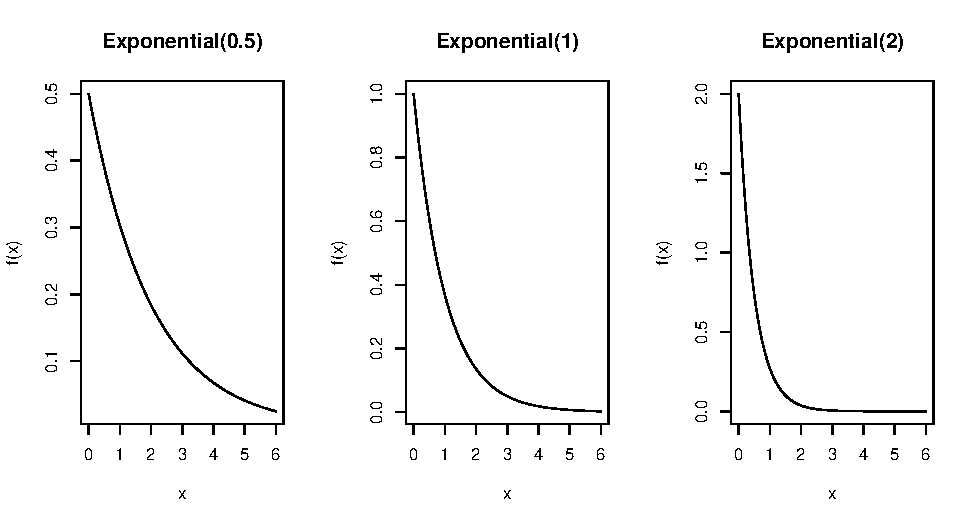
\includegraphics[width=\textwidth]{plots/exponential_shapes.pdf}
	\end{frame}


	\begin{frame}{Exponential Distribution: Example 1}
		Average time required to repair a machine is \(0.5\) hours. What is the probability that the next repair will take more than \(2\) hours?

		\vspace{0.5em}

		Let, \(X\) = time required to repair the machine

		Average time required to repare a machine:
		\[
			\E(X) = \frac{1}{\lambda} a= 0.5 \Rightarrow \lambda = 2
		\]

		Therefore, \(X \sim \mathrm{exponential(2)}\)

		Now, Probability that the next repair will take more than two hours:
		\[
			P(X>2) = \int_{0}^{\infty} 2 e^{-2x} dx = \big[-e^{-2x}\big]_0^{\infty} = \big[-0 + e^{2 \times 2}\big] = e^{-4} = 0.0183.
		\]
	\end{frame}


	\subsection{Normal Distribution}

	\begin{frame}{Normal Distribution}
		A continuous random variable whose distribution is symmetric and bell shaped around its mean is called a normal random variable.

		\vspace{0.5em}

		Let \(X\) be a normally distributed random variable with mean \(\mu\) and variance \(\sigma^2\). It is written as
		\[
			X \sim \mathrm{N}(\mu, \sigma^2)
		\]

		\vspace{0.5em}

		The probability density function of \(X\) is
		\[
			f(x) =
			\frac{1}{\sqrt{2\pi \sigma^2}} \,
			\mathrm{exp}(\frac{(x-\mu)^2}{2\sigma^2}) \, ;
			\quad -\infty < x < \infty
		\]

		\begin{itemize}
			\item \(\E(X) = \mu\)
			\item \(\V(X) = \sigma^2\)
		\end{itemize}
	\end{frame}


	\begin{frame}{Normal Distribution: Shape}
		\centering
		
\includegraphics[width=\textwidth]{plots/normal_shapes.pdf}
	\end{frame}


	\begin{frame}{Properties of Normal Distribution}
		\begin{itemize}
			\item The distribution is symmetric around the mean \(\mu\)
			\item Mean, median and mode are equal
			\item The spread of the distribution depends on the standard deviation \(\sigma\)
			\item Larger \(\sigma\) produces a wider and flatter curve
			\item Total area under the curve is equal to \(1\)
		\end{itemize}
	\end{frame}


	\begin{frame}{Area under the Curve of Normal Distribution: Rule of Thumb}
		For a normal distribution, most of the observations lie close to the mean. The approximate proportions of the data within certain distances from the mean follow a simple rule of thumb.

		\vspace{0.5em}

		\begin{itemize}
			\item About \(68\%\) of the observations lie within one standard deviation of the mean:
			\(
				P(\mu - \sigma < X < \mu + \sigma) \approx 0.68
			\)

			\item About \(95\%\) of the observations lie within two standard deviations of the mean:
			\(
				P(\mu - 2\sigma < X < \mu + 2\sigma) \approx 0.95
			\)

			\item About \(99.7\%\) of the observations lie within three standard deviations of the mean:
			\(
				P(\mu - 3\sigma < X < \mu + 3\sigma) \approx 0.997
			\)
		\end{itemize}

		This result is often referred to as the empirical rule or the 68--95--99.7 or the rule of thumb. 
	\end{frame}


	\begin{frame}{Area under the Curve of Normal Distribution: Rule of Thumb (cont.)}
		\centering
		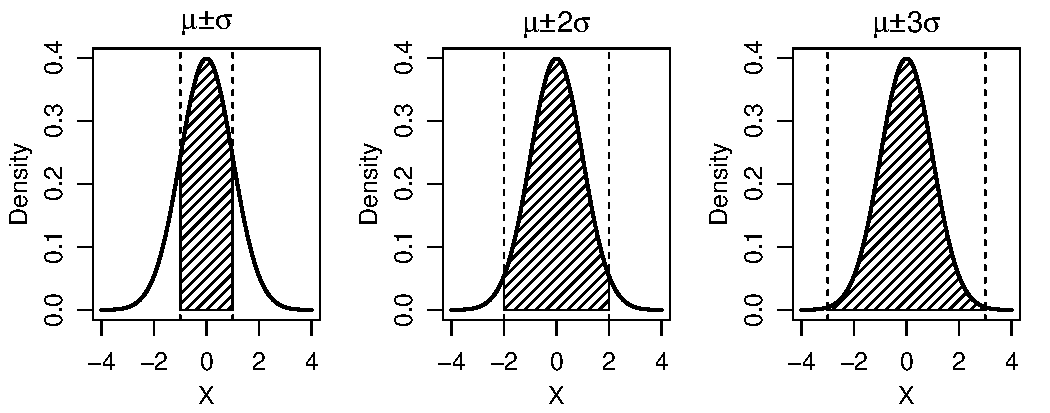
\includegraphics[width=\textwidth]{plots/normal_mu_pm_all_sigma.pdf}
	\end{frame}


	\begin{frame}{Standard Normal Distribution}
		A special case of the normal distribution occurs when the mean is \(0\) and the standard deviation is \(1\).

		\vspace{0.5em}

		If \(X \sim \mathrm{N}(\mu, \sigma^2)\), then the standardized variable
		\[
			Z = \frac{X-\mu}{\sigma}
		\]

		follows the standard normal distribution.

		\vspace{0.5em}

		The standard normal distribution is written as
		\[
			Z \sim \mathrm{N}(0,1)
		\]

		\textbf{\emph{Probabilities for normal variables are usually obtained using standard normal table (Z-table).}}
	\end{frame}


	\begin{frame}{Symmetry of Normal Distribution}
		The normal distribution is symmetric around the mean. Therefore the following relationship holds:
		\begin{columns}
			\begin{column}{0.5\textwidth}
				\begin{align*}
					P(Z <- k) &= P(Z > k) \\
					& = 1 - P(Z < k)
				\end{align*}
				where \(k\) is a positive real number.
				
				\vspace{1em}

				The area under the curve of the highlighted regions are equal.
				\vspace{5em}
			\end{column}
			\begin{column}{0.5\textwidth}
				\centering
				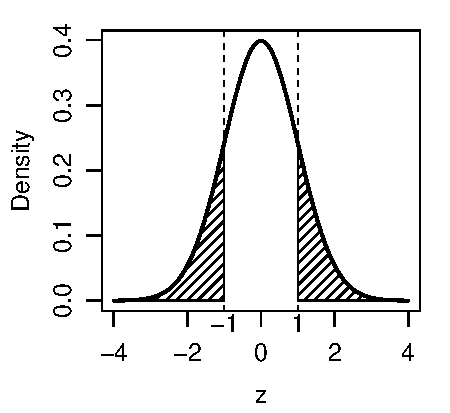
\includegraphics[width=0.95\textwidth]{plots/normal_symmetry.pdf}
			\end{column}
		\end{columns}
	\end{frame}


	\begin{frame}{CDF of the Standard Normal Variable}
		\begin{itemize}
			\item For a normal random variable \(X \sim \mathrm{N}(\mu, \sigma^2)\), probabilities are usually calculated using the standard normal distribution CDF
			\item The cumulative distribution function (CDF) of the standard normal distribution denoted by \(\Phi(x)\) is a function that gives the probability: \(P(Z < z)\)
			\item The Z-table provides the precalculated cumulative probability: \(\Phi(z) = P(Z \leqslant z)\), which represents the area under the standard normal curve to the \textbf{left} of \(z\)
		\end{itemize}
	\end{frame}


	\begin{frame}{Finding Probabilities Using Z-table}
		\begin{itemize}
			\item In order to find probabilities of normally dsitributed random variables we have to perform complex integration to areas under the standard normal curve
			\item However, easier option is to use a calculator/computer or a Z-table
			\item Suppose we need to find the probability: \(P(X < x)\)
			\item First we convert the noraml distribution \(X\) value to to \(Z\) value as: \(z = (x - \mu)/\sigma\)
			\item Then using the table we can find the probability \(\Phi(z) = P(Z < z) = P(X < x)\)
		\end{itemize}
	\end{frame}


	% \begin{frame}{Examples of Probability Regions}
	\begin{frame}{Finding Probabilities Using Z-table}
		The following types of probability regions commonly appear when working with the normal distribution.

		\vspace{0.5em}
		
		Once the value of \(Z\) is obtained, probabilities can be computed using simple rules.

		\begin{itemize}
			\item \(P(Z < z) = \Phi(z)\)
			\item \(P(Z > z) = 1- P(Z < z) = 1 - \Phi(z)\)
			\item \(P(a < Z < b) = P(Z < b)- P(Z < a) = \Phi(b) - \Phi(a)\)
			\item \(P(Z < a \cup Z>b) = P(Z < a) + 1 - P(Z < b) = \Phi(a) + 1 - \Phi(b)\)
			\item \(P(Z > k) = P(Z < -k)\), where \(k\) is a positive real number
		\end{itemize}
	\end{frame}


	\begin{frame}{Normal Distribution: Probability Regions}
		\centering
		
\includegraphics[width=\textwidth]{plots/normal_tail_probabilities.pdf}
	\end{frame}


	\begin{frame}{Normal Distribution: Probability Regions (cont.)}
		\centering
		
\includegraphics[width=\textwidth]{plots/normal_interval_probabilities.pdf}
	\end{frame}


	\begin{frame}{Normal Distribution: Example}
		The heights of students in a university are normally distributed with mean \(170\) cm and standard deviation \(10\) cm.

		\vspace{0.5em}

		Find the following:

		\begin{enumerate}
			\item The probability that a randomly selected student is taller than \(180\) cm
			\item The probability that a student's height lies between \(160\) cm and \(180\) cm
			\item The average height of students
		\end{enumerate}
	\end{frame}


	\begin{frame}{Normal Distribution: Example Solution}
		Let height \(X \sim \mathrm{N}(170, 10^2)\)

		\begin{enumerate}
			\item Probability that a student is taller than \(180\) cm:
			\[
				Z = \frac{180 - 170}{10} = 1
			\]

			\[
				P(X>180) = P(Z>1) = 0.1587
			\]

			\item Probability that height lies between \(160\) and \(180\):
			\[
				Z_1 = \frac{160-170}{10} = -1
			\]

			\[
				Z_2 = \frac{180-170}{10} = 1
			\]

			\[
				P(160<X<180) = P(-1<Z<1) = 0.6826
			\]
		\end{enumerate}

		\vspace{0.5em}

		Average height of students: \(\E(X) = 170\)
	\end{frame}

	
	\section{Approximating Probabilities using the Normal Distribution}


    \section*{Thank you.}

\end{document}